\documentclass[a4paper]{article}
\usepackage{geometry}
\usepackage{booktabs}
\usepackage{cite}
\usepackage{url}
\usepackage[pdftex, final]{graphics}
\title{Pi: A simple unsupervised approach to locating crash-inducing changes}
\author{}
\date{}
\begin{document}

\maketitle

\paragraph{Abstract}
In the process of large software projects evolution, there may be various unexpected errors because of their complexity. One of these severe faults is crash fault that would occur in the usage process by users. Crash faults often occur on these large projects may cause serious consequences. To find the root cause of one crash, developers need to check lots of source codes to locate it, which is a time-consuming and tedious work confusing developers all the time. One feasible solution to the problem is to investigate software changes inducing a crash bug, called crash-inducing changes\cite{ChangeLocator}. By reviewing the these changes, developers can lock the primary cause where the crash was induced more easily. We aim to investigate the most suspicious changes which may be crash-inducing ones to give some cues in solving bugs. In this paper, we propose Pi, a simple method to locate crash-inducing changes without supervised labels. We evaluated Pi with six release versions of Netbeans project. The result show that the recall rate of Pi are close to ChangeLocator while the scores of MAP and MRR are higher than previous one.
\vspace{-1em}

\paragraph{Keywords}
Crash-inducing, Bug localization, Unsupervised approach
\vspace{-1em}


\section{Introduction}

\paragraph{}
Various new features and functions would be integrated together during the long-term evolution of a software. Because of the complexity of application logic and the expansion of software structure, developers would inevitably introduce some unknown errors. The more serious of these bugs are known as crash faults, which would crash in unexpected use procedure. These faults can have a great impact on the user of the software (e.g., property loss, privacy leakage, and even threat to life). Thus, locating the hidden mistakes as soon as possible is very important. Many projects have designed and deployed crash report systems such as Windows Error Reporting\cite{WindowsErrorReport}, Apple Crash Reporter, Mozilla Crash Reports and Netbeans Exception Reports for this purpose. These systems will automatically collect the corresponding crash information from user end when one crash occurs and will allocate them into different buckets to distinguish diverse bugs. A bug is considered to be a serious one that must be fixed when the amount of the crash in a bucket reaches a certain threshold. Developers usually need to check a great number of code to locate the position of the crash occured and then fix it, which is generally a time-consuming and tedious work bothered develop all the time.
\vspace{-1em}

\paragraph{}
A great deal of bug localization techniques(BugLocator\cite{BugLocator}, BLUiR\cite{BLUiR}, BRTracer\cite{BRTracer}) based on bug report has been proposed to facilitate software repair process. These methods locate the bug at the source file level, which refer to a bug report and source files as a query and a set of docuemnts. They calculate the suspicious score according to the similarity between the query and the documents, and then send the developer a list of descending order files according to these scores. The files in front of the list are more likely to contain the specified bug. From the experimental results, these methods get some satisfied results in the case where the quality of source codes and reports are both good.
\vspace{-1em}

\paragraph{}
Another direction of research in bug localization is to review the bug-inducing changes. Wen et al.\cite{Locus} found that to understand and fix a certain bug, developers often refer to the bug inducing changes in the discussion of bug reports. Although some approaches(e.g., Locus\cite{Locus}, ChangeLocator\cite{ChangeLocator}) have been proposed, we found that the existing approaches still exists some issues well, leading to an undesirable effect.
\vspace{-1em}

\paragraph{}
In this paper, We design a simple unsupervised method, called Pi, to locate crash-inducing changes which is at commit level given buckets of crash reports by computing the position of changes and the relativity with components the bug exists. To evaluate Pi, we conduct an experimental study using data from six release versions of NetBeans project. The result show that the recall rate of Pi are close to ChangeLocator while the scores of MAP and MRR are higher than previous one.
\vspace{-1em}

\paragraph{}
The remainder of this paper is organized as follows. First, we briefly introduce the existing approach in Section 2. Section 3 presents our proposed Pi approach in details. We then design our experiment in Section 4 and show the evaluation results in Section 5. In Section 6 and Section 7, we discuss issues involved in our approach and the threats to validity, respectively. We illustrate the related work in Section 8 and conclude this paper in Section 9.
\vspace{-1em}


\section{Existing approach}

\paragraph{}
Various bug localization approaches has been proposed before to improve the effect of localization, such as the traditional IR based approach using VSM model and its different variants(e.g., rVSM with similar bug reports\cite{BugLocator}, rVSM with structured information\cite{BLUiR}, rVSM with stack trace\cite{BRTracer}), bug-inducing changes based methods(e.g., Locus\cite{Locus}, ChangeLocator\cite{ChangeLocator}), etc. The rest of this section is the details introduction.
\vspace{-1em}

\subsection{IR based approach}
\paragraph{}
In early years, many researchers have porposed information retrieval(IR) techniques to locate relevant source files based on given bug report automatically\cite{BugLocator}. IR based methods consider a bug report as a query and rank the source files by computing their relevance to the query. The most popular model used for IR methods is called VSM(e.g., Vector Space Model), which is a matrix model that each row denotes a query and each column as a source code document, and each element of which is represented by \emph{tf-idf}. These IR based approaches don't need program execution information so that their analysis is simple and easy to implementation.
\vspace{-1em}

\paragraph{}
Whereas, the effect of method purely using VSM model is not just as one wishes, thus, researchers proposed many different revised variants to boost the rank performance. Zhou et al.\cite{BugLocator} take the length of source file into consideration and argue that the information about similar bug reports that have been fixed before is useful to locate a bug. According to their research, larger source code files tend to have higher probability of containing a bug and the assumption about similar bugs is that similar bugs tend to fix similar files. 
\vspace{-1em}

\subsection{Bug-inducing changes based approach}
\paragraph{}
According to Wu et al.'s\cite{ChangeLocator} investigation, bug-inducing changes is a good indicator to fix a bug. They summarize that developers can obtain four primary benefits by checking and understanding bug-inducing changes. First, a developer who committed specific bug-inducing changes is familiar with the corrsponding buggy source code that need be fixed. Second, the contextual clues underlying in a bug-inducing change is more easily to find so that develop can get more helpful information about how to fix the bug. A bug, moreover, may be fixed very conveniently just by reverting bug-inducing changes and 1069 bugs in NetBeans project was fixed following the opeartor. They also found that \emph{automatic program repair techniques} can greatly benefited from the ability to locate the bug inducing changes. Based on these researches of bug-inducing changes, they implemented their technique as a tool call ChangeLocator.
\vspace{-1em}

\paragraph{}
The research results of Wu et al's empirical study also suggest that one can narrow down the candidate set of the crash-inducing changes based on crash reports. Futhermore, crash-inducing changes exhibit certain characteristics. Crash-inducing changes usuallly appear closer to the crash point that is the crash occured and a change is more likely to be a inducing one if the change modified the lines near to the crashing lines. In addition, Crash-inducing changes for a bucket appear frequently in the crash reports of that bucket, and those changes that appear in multiple buckets are less likely to be crash-inducing changes. And that, The change affects the source files in the component where the bucket of crash reports happened is more likely to be a crash-inducing change for that bucket. Finally, the committed time of crash-inducing changes is closer to the reporting time of the crashes.
\vspace{-1em}


\section{Pi approach}
\paragraph{}
As mentioned before, we build our two heuristic metrics in Pi.
\vspace{-1em}


\section{Experimental design}
\paragraph{}
This section describes our experimental design for evaluating Pi. We first introduce the experimental setup. Then, we describe the metrics. After that, we present the research questions.
\vspace{-1em}

\subsection{Experimental Setup}
\paragraph{}
We choose the large-scale projects, namely NetBeans\footnote{https://netbeans.org/}​, as our evaluation subjects. The details of the dataset are listed in Table \ref{NetBeansProject}.
\vspace{-1em}

\begin{table}[!htbp]
\centering
\caption{Six released NetBeans subject for evaluation }\label{NetBeansProject}
\begin{tabular}{ccccc}
\toprule
Released Version & \#Files & KLOC & \#Revs & \#Buckets \\
\midrule
Netbeans 6.5 & 25,558 & 5,524 & 110,887 &  42 \\
Netbeans 6.7 & 48,044 & 10,331 & 139,189 & 61 \\
Netbeans 6.8 & 499,18 & 10,717 & 158,936 & 52 \\
Netbeans 6.9 & 53,264 & 11,632 & 176,495 & 40 \\
Netbeans 7.0 & 46,189 & 9,745 & 196,886 & 38 \\
Netbeans 7.1 & 38,900 & 8,429 & 217,206 & 41 \\
Netbeans 7.2 & 39,674 & 8,666 & 235,526 & 39 \\
\bottomrule
\end{tabular}
\end{table}


\subsection{Evaluation Metrics}
\paragraph{}
Just like ChangeLocator, Pi will produce a ranked list of all changes according to their suspicious score. Developers can check the changes from the top of list and find out the location where crash occured. In order to evaluate the effectiveness of Pi, we adopt the following three metrics, which are widely used to evaluate the performance of ranking relevant tecchniques.\\
\vspace{-1em}

\begin{itemize}
\item \textbf{Recall@K}
This metric reports the percentage of bugs.
\item \textbf{MRR}
This metric is used to evaluate the ability to locate the first relevant code element for a bug.
\item \textbf{MAP}
The metric provides a single-figure measure of quality across recall levels. This metric is used to evaluate the ability of approaches to locate all the buggy entities of a bug.
\end{itemize}


\subsection{Research Questions}


\section{Experimental result}

\scalebox{0.8}[0.8]{\centering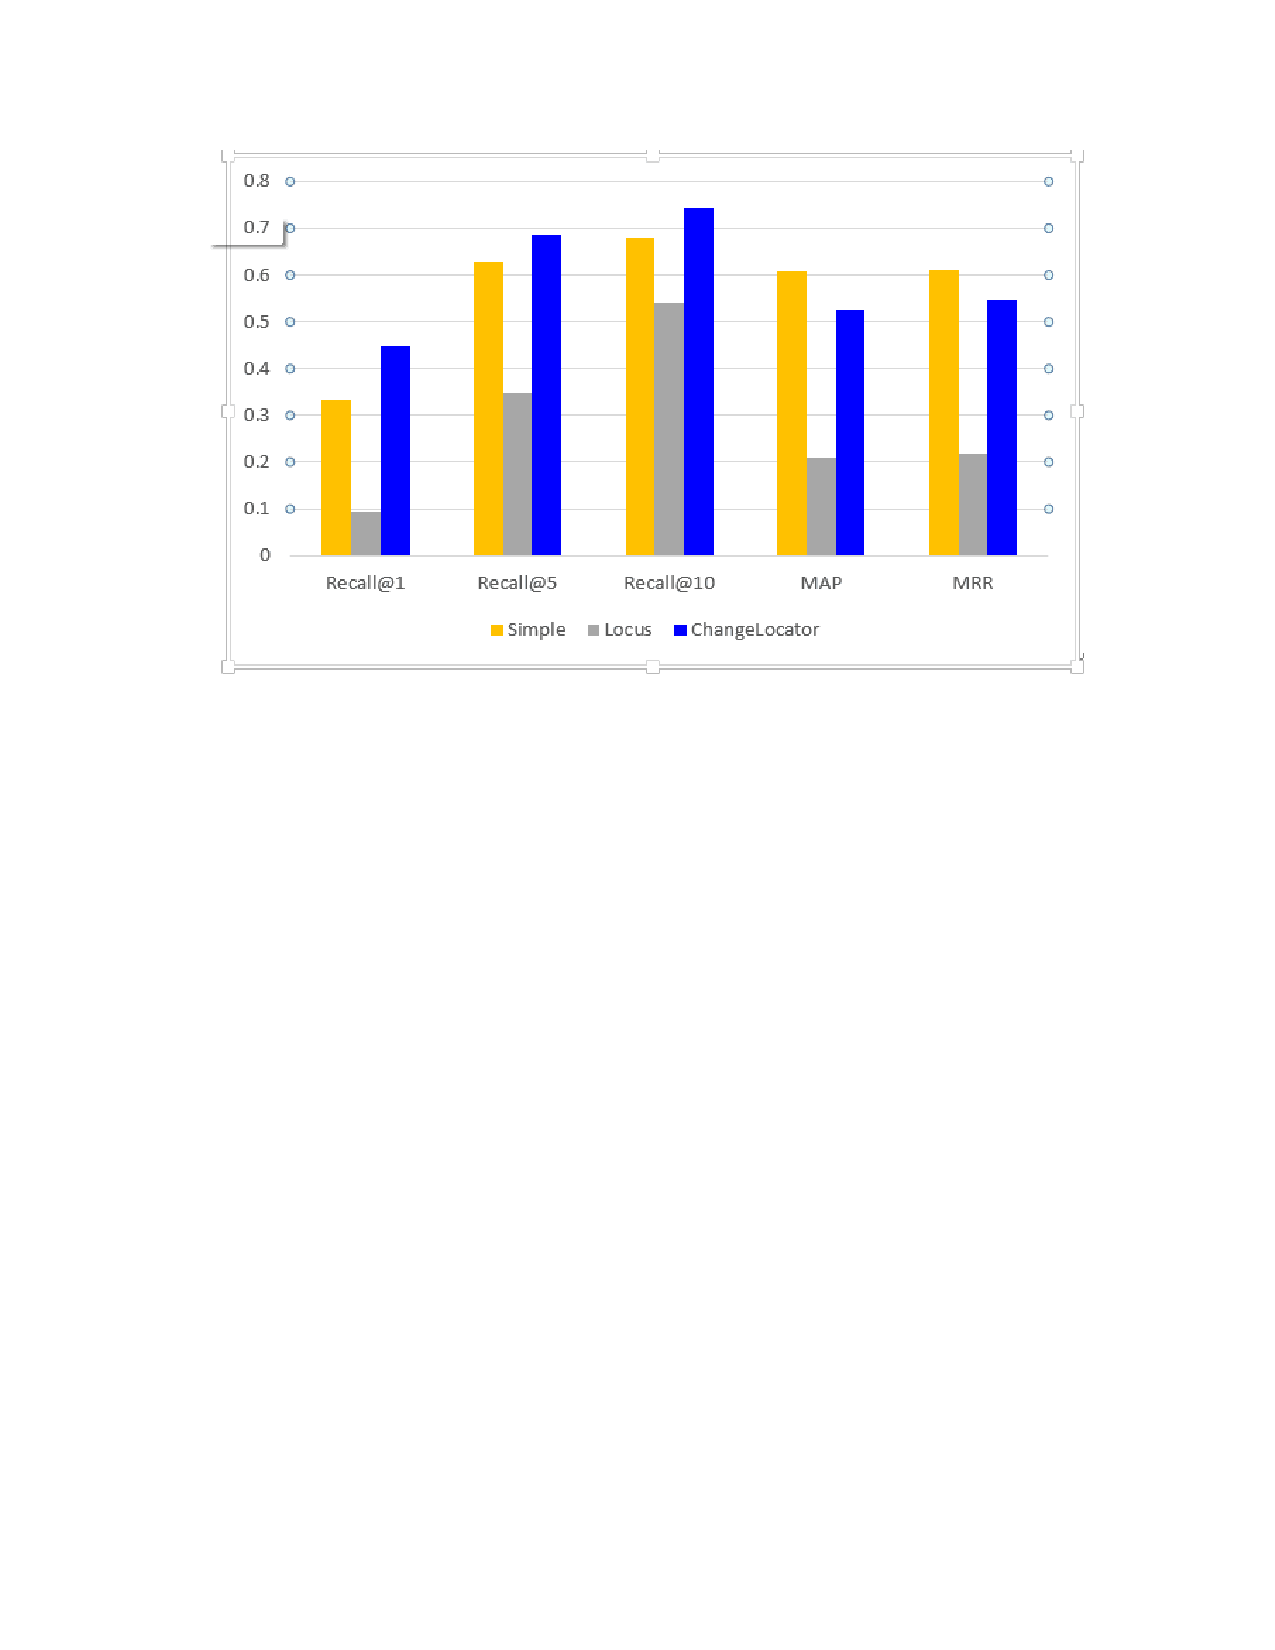
\includegraphics{compare.pdf}}

\section{Discussions}



\section{Threats to validity}



\section{Related work}



\section{Conclusions}


\section{Acknowledgments}
\paragraph{}
We would like to thank Wu et al.\cite{ChangeLocator} , who collect the NetBeans project dataset.


\bibliographystyle{plain}
\bibliography{cited}

\end{document}